This is an output-only problem. That means, that you don't need to submit your solution, but only need to submit outputs for given set of inputs. You can download test data in a problem materials section. It is an archive containing input files 01, 02, 03, \dots. You need to submit a single zip-archive containing your outputs 01.out, 02.out, 03.out, \dots in the root of the archive.  An archive can contain no answers for some of tests, you'll receive ``\t{Wrong Answer}'' verdict in these tests.

Two undirected graphs $G$ and $H$ are said to be isomorphic if: 

\begin{itemize}
    \item they have the same number of vertices;
    \item a one-to-one correspondence exists between their vertices so that, for any two distinct vertices of $G$, there exists an edge between them if and only if there exists an edge between their corresponding vertices in $H$. .
\end{itemize}

For example, the next two graphs are isomorphic, even though they look different here: 

\begin{center}
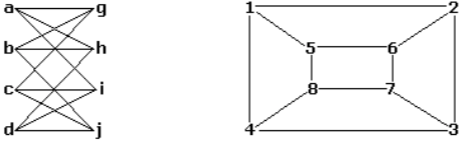
\includegraphics{pic1.png}
\end{center}

A possible one-to-one correspondence showing that these two graphs are isomorphic is given by \t{\{a--1, b--6, c--8, d--3, g--5, h--2, i--4, j--7\}},
but others exist too.

A subgraph of a graph $G$ is a graph whose sets of vertices and edges are subsets of those in $G$. Note that $G$ is a subgraph of itself. The following example shows a graph and one of its subgraphs:

\begin{center}
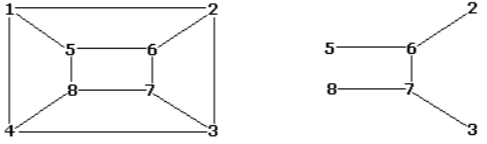
\includegraphics{pic2.png}
\end{center}

We say that a graph $G$ contains another graph $H$ if there is at least one subgraph $H'$ of $G$ which is isomorphic to $H$. The following figure shows a graph $G$ that contains the graph $H$. 

\begin{center}
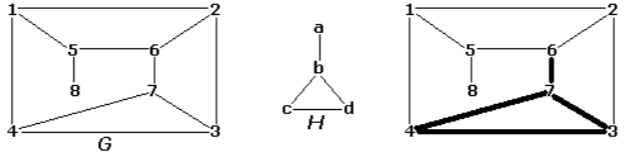
\includegraphics[scale=0.7]{pic3.png}
\end{center}

Given two undirected graphs $G$ and $H$, produce a subgraph $G'$ of $G$ such that:

\begin{itemize}
\item the number of vertices in $G$ and $G'$ is the same;
\item $H$ is not contained in $G'$.
\end{itemize}

Naturally, there may be many subgraphs $G'$ with the above properties. Produce one of those subgraphs with as many edges as possible. 
